%%Bài toán đề xuất bởi NVPL

\textbf{Enzyme cứng hay mềm?}

\textit{Enzyme} là các protein có tác dụng làm chất xúc tác chuyển hoá về mặt hoá học các phân tử liên kết với chúng. Enzyme không tạo ra phản ứng mới hoặc thay đổi chiều hướng của phản ứng hoá học, chúng chỉ thúc đẩy hoặc ức chế các quá trình tự phát. Đôi khi việc tăng tốc phản ứng của enzyme còn mạnh hơn gấp hàng triệu lần so với việc tăng tốc bởi các chất xúc tác hoá học mạnh nhất. Trong bài tập này, ta sẽ sử dụng các mô hình cơ học cổ điển đơn giản nhất để tư duy trực quan về tính chất của enzyme.

\begin{enumerate}
    \item \textbf{Enzyme cứng hay mềm?}\\
    Quá trình xúc tác của enzyme bao gồm ba trạng thái như sau \textbf{(Hình 1)}:
    \begin{enumerate}
        \item \textbf{Trạng thái đầu:} \textit{Cơ chất (Substrate)} di chuyển đến \textit{vùng hoạt động (active site)} của enzyme và liên kết với enzyme để hình thành phức hệ enzyme - cơ chất. 
        \item \textbf{Trạng thái chuyển tiếp:} Enzyme xúc tác phản ứng biến đổi \textit{Cơ chất (Substrate)} thành \textit{Sản phẩm (Product)}, tạo thành phức hệ enzyme - sản phẩm.
        \item \textbf{Trạng thái cuối:} Enzyme thực hiện chức năng "nhả phối tử", giải phóng \textit{Sản phẩm (Product)} khỏi enzyme.
    \end{enumerate}
\begin{center}
    \begin{figure}[htp]
    \begin{center}
        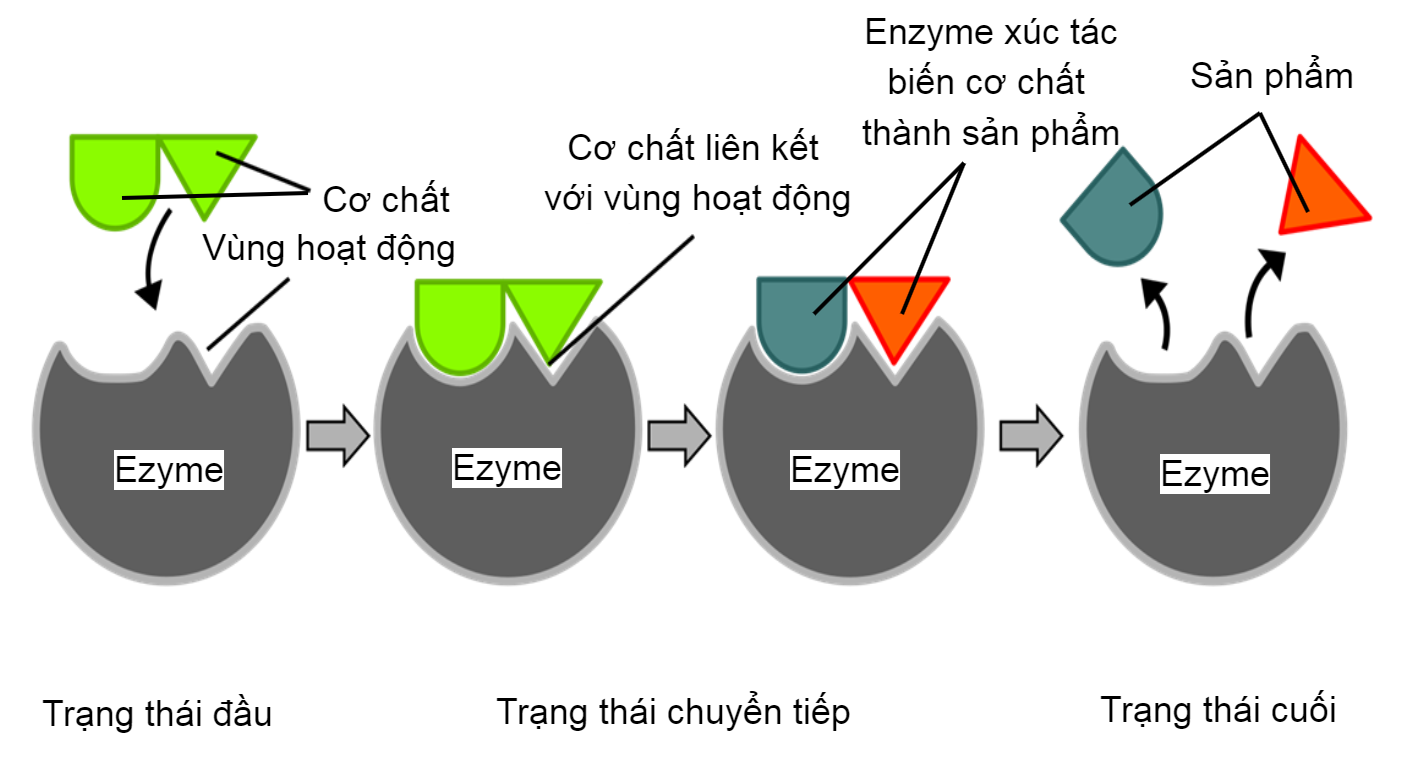
\includegraphics[scale=.23
        ]{Problem_5/image/1.png}
    \end{center}
    \begin{center}
    Hình 1: Các trạng thái của enzyme trong quá trình xúc tác.
    \end{center}
    \end{figure}
\end{center}
    Trong bài toán này, ta sẽ khảo sát tính chất của \textit{abzyme (anti-body enzyme hay enzyme kháng thể)} trong trạng thái chuyển tiếp. Lý do ta chọn abzyme mà không phải ezyme tự nhiên là để đơn giản hoá các tương tác do abzyme không liên kết với cơ chất bằng liên kết cộng hoá trị. Ta xét mô hình cơ học đơn giản \textbf{(Hình 2)}, giả sử hai phân tử (phải hình thành liên kết hoá học) - đại diện cho cơ chất - được kéo vào vùng hoạt động của abzyme (kẽ hở). Cơ chất được mô hình hoá như những quả bóng nhỏ có đường kính $d$ và kẽ hở có độ rộng ban đầu là $a$; để tạo điều kiện hình thành liên kết phức hệ enzyme - cơ chất, hệ này sẽ hấp thụ năng lượng để các quả bóng bị nén lại và kẽ hở mở rộng ra ($a<2d$). Cả abzyme và cơ chất đều có tính đàn hồi và tuân theo định luật Hooke, hệ số đàn hồi của abzyme ở vùng hoạt động là $k_e$, hệ số đàn hồi của cơ chất là $k_s$. Coi tất cả biến dạng chỉ đáng kể trên phương $x$ và bỏ qua biến dạng theo các phương khác như trên hình và bỏ qua động năng của toàn hệ. Cho biết, một enzyme xúc tác càng hiệu quả sẽ tiêu tốn càng ít năng lượng cho việc biến dạng chính nó. 
    \begin{enumerate}[label=\textbf{\alph*,}]\itemsep0em
        \item Xác định biểu thức năng lượng cần cung cấp cho abzyme và cơ chất.
        \item Một enzyme hoạt động hiệu quả sẽ phải thật "cứng" hay thật "mềm"?
    \end{enumerate}
    \begin{center}
    \begin{figure}[htp]
    \begin{center}
        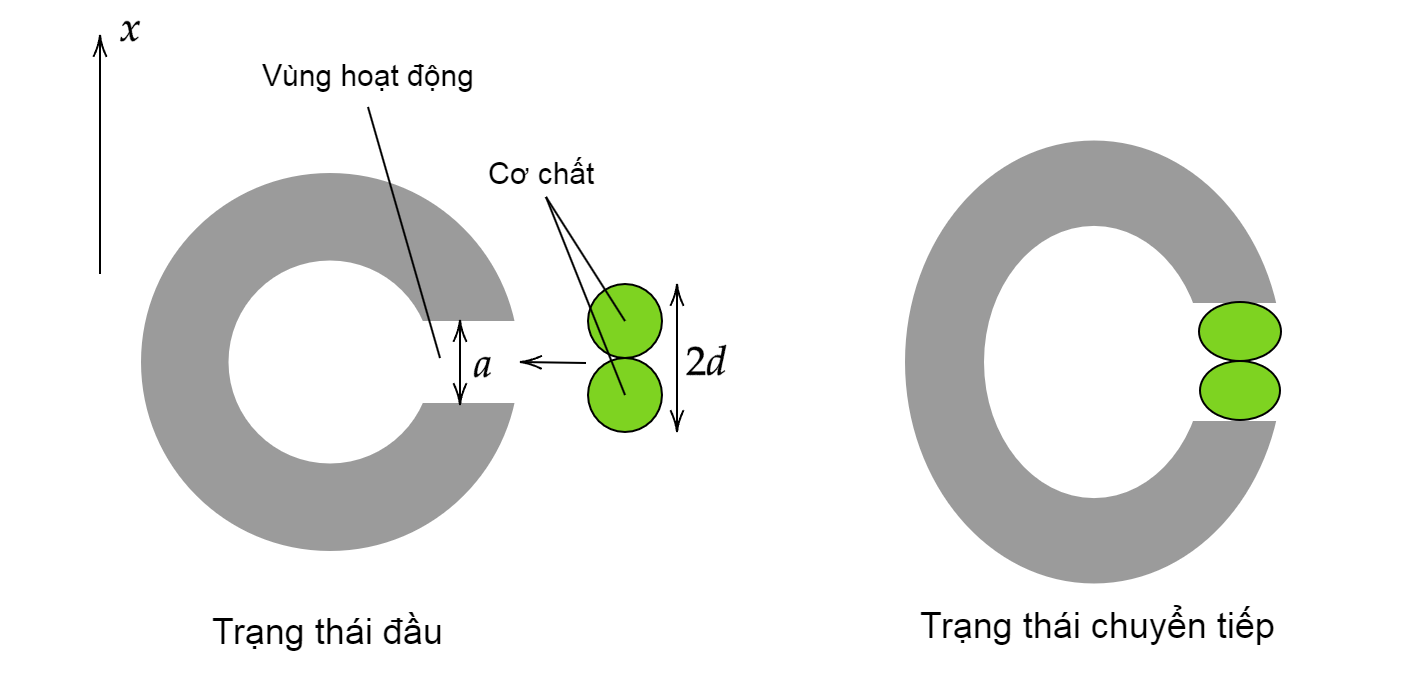
\includegraphics[scale=.23
        ]{Problem_5/image/2.png}
    \end{center}
    \begin{center}
    Hình 2: Mô hình cơ học đơn giản.
    \end{center}
    \end{figure}
\end{center}
\item \textbf{Bỏ qua động năng?}\\
    Trong phần trước ta đã bỏ qua hoàn toàn động năng của hệ, nói cách khác, ta coi hệ enzyme là tĩnh hoặc gần tĩnh, vậy trên thực tế điều này có đúng không ? Giả sử enzyme có động năng, chẳng hạn động năng trong quá trình dao động. Xét một enzyme dao động theo phương $x$ trong môi trường nhớt (chẳng hạn là nước hay màng), enzyme có khối lượng riêng là $\rho \approx 1 \ \si{g/cm^3}$, để cho đơn giản, coi enzyme có các kích thước tuyến tính về bậc độ lớn với đường kính $D$ của nó (tiết diện $S \sim D^2$, thể tích $V \sim D^3$) và $D \approx 4 \ \si{nm}$. Enzyme chịu lực đàn hồi do biến dạng tuân theo định luật Hooke, lực đàn hồi có biểu thức là:
    $$F_{\text{ela}}=-\dfrac{ES}{D}x.$$
    Trong đó S là tiết diện và $E$ là suất đàn hồi, $E \approx 10^{10} \ \si{g \cdot cm^{-1} \cdot s^{-2}}$.\\
    Để cho đơn giản, chọn gốc thời gian tại $t=0$, coi enzyme ở thời điểm $t=0$ có vận tốc $v(0)=0$ và li độ $x(0)=x_0$.
    \begin{enumerate}[label=\textbf{\alph*,}]\itemsep0em
        \item Giả sử bỏ qua ma sát nhớt tác dụng lên cấu trúc enzyme trong quá trình dao động, hãy xác định chu kỳ dao động $T_0$ của enzyme.
        \item Trên thực tế, quá trình dao động của enzyme trong môi trường nhớt enzyme chịu thêm lực ma sát nhớt tuân theo định luật Stokes, có biểu thức là:
        $$F_{\text{vis}}= -10 \eta D \dfrac{dx}{dt}.$$
    Trong đó $\eta$ là độ nhớt của môi trường, $\eta \approx 0.01 \ \si{g\cdot cm^{-1}\cdot s^{-1}}$.\\
    \begin{enumerate}
        \item Viết biểu thức li độ phụ thuộc thời gian $x(t)$.
        \item Tại thời điểm $t=T_0$ và $t=2T_0$, li độ $x$ lần lượt bằng bao nhiêu lần li độ $x_0$ tại thời điểm ban đầu. Từ đó đưa ra nhận xét về sự thay đổi của hiện tượng khi tính đến ma sát nhớt.
    \end{enumerate}
    \end{enumerate}
\end{enumerate}

\begin{flushright}
    (Biên soạn bởi Nhân viên phòng lab)
\end{flushright}